\begin{frame}{Matrix struct}
\begin{itemize}
    \item ptr
    \item rows and cols
    \item stride
\end{itemize}
\end{frame}

\begin{frame}[fragile]{Matrix functions}
    \begin{lstlisting}
DATA* matrix_index(Matrix m, int i, int j)
Matrix up(Matrix m);
Matrix down(Matrix m);
Matrix left(Matrix m);
Matrix right(Matrix m);
//...
    \end{lstlisting}

    \begin{columns}[T]
        \begin{column}{0.495\textwidth}
            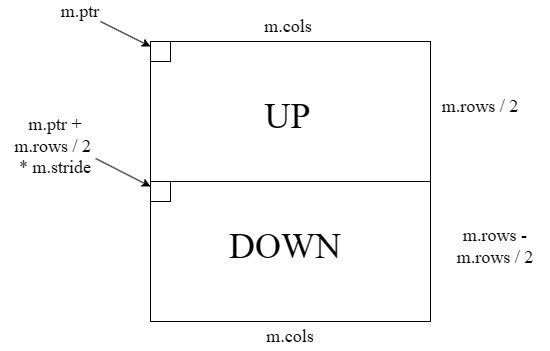
\includegraphics[width=\textwidth]{Images/matrix_split.png}
        \end{column}

        \begin{column}{0.495\textwidth}
            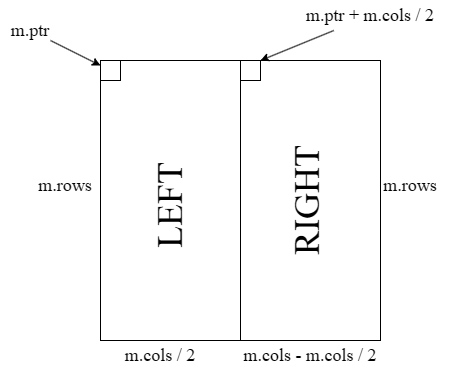
\includegraphics[width=0.7\textwidth]{Images/left_right_split.png}
        \end{column}
    \end{columns}
\end{frame}